
\documentclass[12pt,oneside]{report}
\usepackage[T1]{fontenc}		% Einstellungen fuer Umlaute usw.
\usepackage[utf8x]{inputenc}
\usepackage[ngerman]{babel}

\usepackage{parskip}			% Einstellungen fuer Absaetze: Abstand statt Einrueckung

\usepackage[a4paper,			% Papierformat A4
	    left=2.5cm,				% linker Rand
	    right=2.5cm,			% rechter Rand
	    top=1.5cm,				% oberer Rand
	    bottom=1.5cm,			% unter Rand
	    marginparsep=5mm,		% Abstand der Randnotizen
	    marginparwidth=10mm, 	% Breite der Randnotizen
	    headheight=7mm,			% Hoehe der Kopfzeile
	    headsep=1.2cm,			% Abstand der Kopfzeile
	    footskip=1.5cm,			% Abstand der Fusszeile
	    includeheadfoot]{geometry}

\usepackage{fancyhdr}						% Konfiguration von Kopf- und Fusszeilen
\pagestyle{fancy}							% Seitenstil 'fancy'
\fancyhf{}									% vorhandene Einstellungen loeschen
\setlength{\headwidth}{\textwidth}			% Kopf- und Fusszeile so breit wie der Haupttext
\fancyfoot[R]{\thepage} 					% Festlegung des Seitenstils: Seitenzahlen in der Fusszeile rechts
\fancyfoot[L]{\leftmark}					% Kapitelnr. und -Bezeichnung in der Fusszeile links
\fancyhead[R]{\IhreArbeit}					% "Bachelorarbeit" in der Kopfzeile rechts
\fancyhead[L]{\IhrVorname\ \IhrNachname}	% Vorname und Name in der Kopfzeile links
\renewcommand{\chaptermark}[1]{			% Definition der Ausgabe des Kapitels
  \markboth{Kapitel \thechapter. #1}{}}
\renewcommand{\headrulewidth}{0.5pt}		% Trennlinie zwischen Kopfzeile und Haupttext
\renewcommand{\footrulewidth}{0.5pt}		% Trennlinie zwischen Haupttext und Fusszeile
\fancypagestyle{plain}{					% Anpassung des Seitenstils 'plain' bei Beginn neuer Kapitel
  \fancyhf{}								% Vorbelegung loeschen
  \fancyfoot[C]{\thepage}					% Seitenzeilen in der Fusszeile mittig
  \fancyhead[R]{\IhreArbeit}				% "Bachelorarbeit" in der Kopfzeile rechts
  \fancyhead[L]{\IhrVorname\ \IhrNachname}	% Vorname und Name in der Kopfzeile links
}

\usepackage{amsmath}			% Pakete fuer den Mathematikmodus
\usepackage{amssymb}
\usepackage[intlimits]{empheq}

\usepackage[sc]{mathpazo}		% Schriftart Palatino fuer Haupttext und Mathematikmodus
\usepackage{pifont}				% zusaetzliche Symbole

\usepackage[format=hang,		% Einstellung fuer Bildunterschriften
            font={footnotesize},
            labelfont={bf},
            margin=1cm,
            aboveskip=5pt,
            position=bottom]{caption}

\usepackage{graphicx}							% Einbinden von Graphiken
\usepackage[svgnames,table,hyperref]{xcolor} 	% Verwendung von Farben
\usepackage{tikz}								% Erstellen von Grafiken
\usetikzlibrary{positioning,arrows,plotmarks} % TikZ-Bibliotheken







%\usepackage{pgfplots}  % Darstellung von Plots, Funktionen, Graphen usw.

%
% Weitere Pakete
%
%\usepackage{listings}			% Darstellung von Quellcode
% configure your listings style
\usepackage{listings}
\lstset{
	tabsize=3,
	extendedchars=true,
	frame=single,
	showstringspaces=true,
	numbers=left,
	numberstyle=\small,
	breakautoindent=true
}
%\lstset{language=Python, basicstyle=\ttfamily, numbers=none}
%
%\usepackage[european, siunitx]{circuitikz}	% Darstellung von Schaltungen
%
%\usepackage{enumerate}			% Formatierung nummerierter Listen

\usepackage{microtype,relsize}					% Wird verwendet, um Nachnamen auf Titelseite gesperrt darzustellen
\newcommand*{\Sperren}[1]{\textls*[100]{#1}}

% 
% Persoenliche Angaben
% 
\newcommand*{\IhrVorname}{Patrick}
\newcommand*{\IhrNachname}{Sabau}
\newcommand*{\IhrStudiengang}{Künstliche Intelligenz (Master)}
\newcommand*{\IhreArbeit}{Studienarbeit Deep Vision}
\newcommand*{\IhrTitelDE}{Hand Pose Estimation}
\newcommand*{\IhrBearbeitungszeitraumVON}{25. Mai 2022}
\newcommand*{\IhrBearbeitungszeitraumBIS}{01. Juli 2022}
\newcommand*{\IhrErstpruefer}{Prof. Dr. phil. Tatyana Ivanovska}




%\usepackage[bookmarks, raiselinks, pageanchor, % PDF-Einstellungen
%            hyperindex, colorlinks,
%            citecolor=black, linkcolor=black,
%            urlcolor=black, filecolor=black,
%            menucolor=black]{hyperref}
% pdf hyperref
\usepackage[
    bookmarks=true,
    bookmarksopen=true,
    bookmarksnumbered=true,
    bookmarksopenlevel=1,
    pdfpagelabels=true,
    colorlinks=true,
    linkcolor=red,
    urlcolor=magenta,
    anchorcolor=black,
    citecolor=cyan,
    filecolor=magenta,
    menucolor=red,
    plainpages=false,
    hypertexnames=true,
    linktocpage=true,
    ]{hyperref}
\hypersetup{pdftitle={\IhrTitelDE},%
            pdfauthor={\IhrVorname\ \IhrNachname}}

%
% Beginn des Textteils
%
\begin{document}
  \pagenumbering{roman}
  %\begin{titlepage}					% Titelseite
  %  \thispagestyle{empty}
  %  \begin{center}
  %    \Large
  %    Ostbayerische Technische Hochschule Amberg-Weiden\\
  %    Fakultät Elektrotechnik, Medien und Informatik\\[1cm]
  %    Studiengang \IhrStudiengang\\[1cm]
  %    \textbf{\IhreArbeit}\\[1cm]
  %    von\\[1cm]
  %    \IhrVorname\ \Sperren{\textbf{\IhrNachname}}\\[1cm]
  %    \textbf{\IhrTitelDE}\\[1cm]
  %  \end{center}
  %\end{titlepage}
  %\clearpage
  \thispagestyle{empty}			% 1. Seite soll eine Leerseite sein (dazu muss ein Trick verwendet werden)
  \mbox{}
  %\clearpage
  \thispagestyle{empty}			% 2. Seite wie Titelseite, aber mit zusaetzlichen Angaben
  \begin{center}
    \Large
    Ostbayerische Technische Hochschule Amberg-Weiden\\
    Fakultät Elektrotechnik, Medien und Informatik\\[1cm]
    Studiengang \IhrStudiengang\\[1cm]
    \textbf{\IhreArbeit}\\[1cm]
    von\\[1cm]
    \IhrVorname\ \Sperren{\IhrNachname}\\[1cm]
    \textbf{\IhrTitelDE}\\[1cm]
  \end{center}
  \vspace*{5cm}
  \begin{tabbing}
    \underbar{Bearbeitungszeitraum:}\qquad\= von\qquad\=\IhrBearbeitungszeitraumVON\\
                                          \> bis      \>\IhrBearbeitungszeitraumBIS
  \end{tabbing}
  \vspace*{1cm}
  \underbar{Prüfer:}\qquad\IhrErstpruefer\par 
  %\clearpage
  %\include{formblatt_para12apo}		% 3. Seite: Formblatt Bestaetigung nach Paragraph 12 APO
  %\include{formblatt_summary}			% 4. Seite: Formblatt Zusammenfassung
  \thispagestyle{empty}	
  \tableofcontents
  \newpage
  %\chapter*{Symbole, Formelzeichen und Einheiten}
  %\newpage
  
  
  \pagenumbering{arabic}
  
  \chapter{Einleitung}\label{einleitung}

Bildverarbeitung ist heutzutage für den durchschnittlichen Bürger immer noch ein nicht vertrauter Begriff. 
Jedoch sind viele Menschen durch Themen wie autonomes Fahren oder auch Instagram-Filter mit diesem Thema in Berührung getreten.
Allerdings bietet dieser Themenbereich ein viel größeres Potenzial, als weitläufig bekannt ist.
Dieses Projekt zeigt einen diese Potenziale: Pose Estimation von (interagierenden) Händen. \newline
Pose Estimation beschreibt dabei, das extrahieren der Lage sogenannter Schlüsselpunkte (Keypoints).
Diese 2D oder auch teilweise 3D Koordinaten können aus unterschiedlichen Quellen extrahiert werden, von simplen 2D RGB Bildern bis hin zu komplexer Sensorik wie Lidar. \newline
OpenPose \cite{openpose} ist beispielsweise ein Projekt, welches 2D Koordinaten eines gesamten menschlichen Körpers erkennt, wohingegen es auch Versuche gibt, nur einzelne Körperteile, wie z.B. Hände, genauer zu betrachten. 
Für Hände gibt es eine Vielzahl an Datensätzen und Modellen.
Diese können in der Größe (Anzahl der Datenpunke), der Erstellung (Kameraaufnahmen oder synthetische 3D Modelle) oder auch in der Art der Labels (2D und/oder 3D) variieren. 
Hier ein paar Beispiele:
\begin{itemize}
\item FreiHand: RGB Bilder aus verschiedenen Kamerarblickwinkeln \cite{freihand}
\item Ego3D: synthetische Bilder aus der Ego-Perspektive \cite{ego3d}
\item BigHand2.2M: Tiefenbilder mit 3D Koordinaten \cite{bighand}
\end{itemize}

Im Folgenden wird ein im Jahr 2020 erschienener Datensatz InterHand2.6M \cite{InterHand} genutzt um 2D Pose Estimation an einzelnen und auch interagierenden Händen zu entwickeln.
Dieser Datensatz wurde von Meta (damals noch Facebook) veröffentlicht. Ein möglicher Use Case, der für das Unternehmen relevant ist, ist die 3D Erkennung der Hände um diese dann mittels Virtual Reality im sogenannten 'Metaverse' korrekt zu visualisieren.
  \chapter{Datensatz}

Wie bereits in Chapter \ref{einleitung} erwähnt, wird der InterHand2.6M Datensatz \cite{InterHand} genutzt.
Dabei handelt es sich um Bilder von Händen, die zeitgleich von 6 verschieden Kameras aus unterschiedlichen Perspektiven aufgenommen wurden. \\
\begin{figure}[!htb]
    \centering
    \fbox{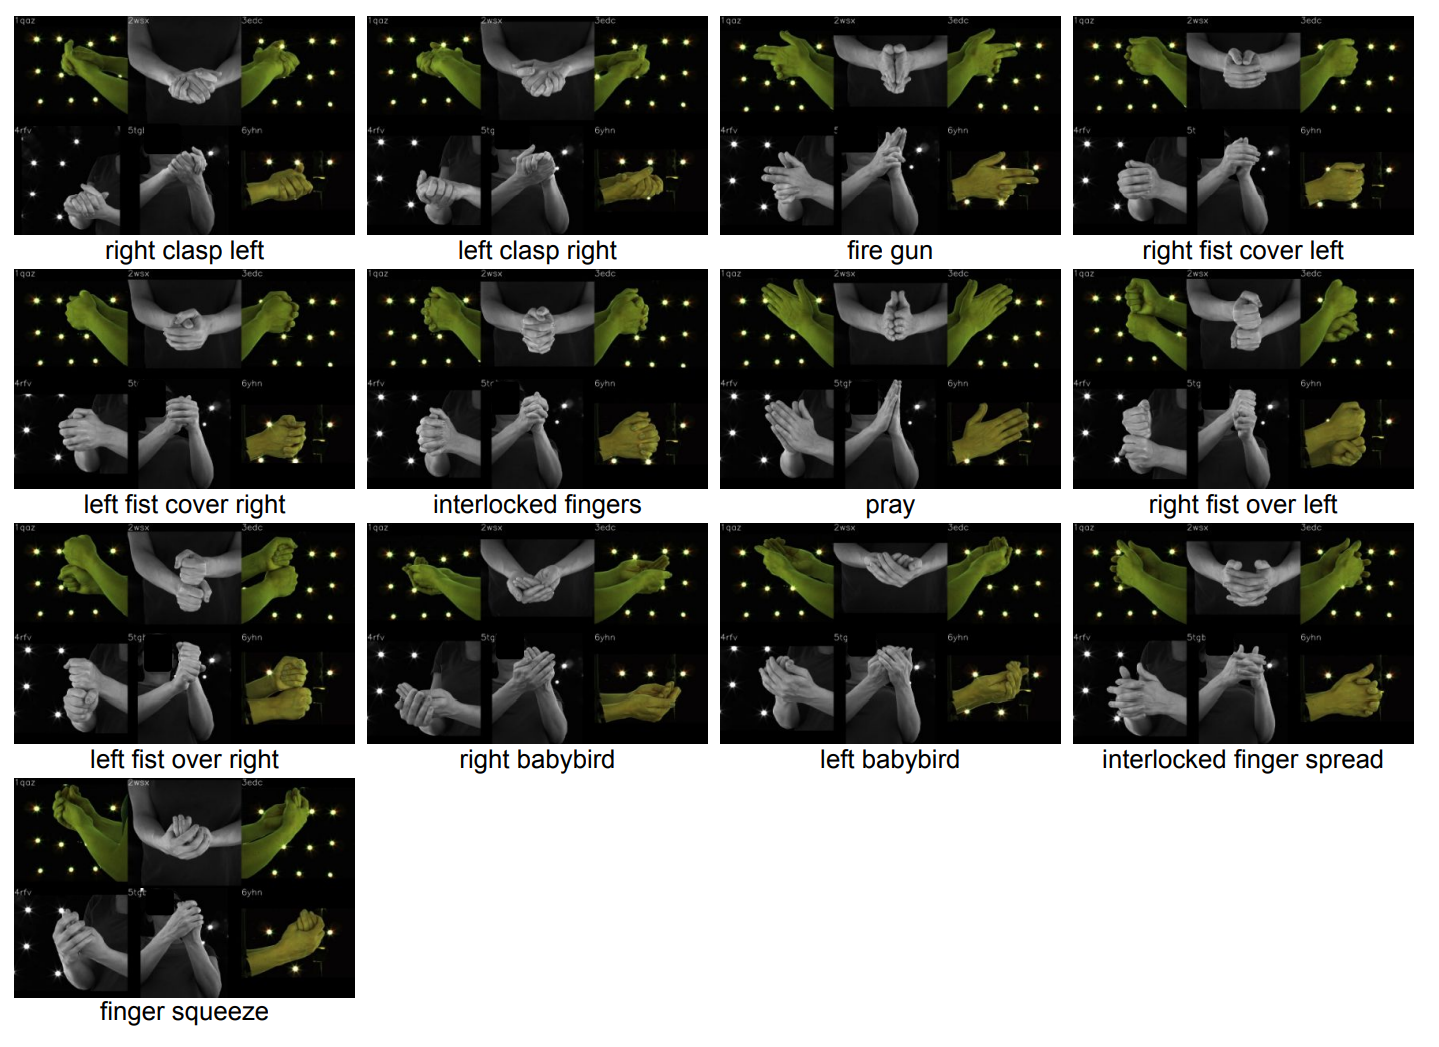
\includegraphics[width=15.5cm]{abbildungen/interhand26.PNG}}
    \caption{Beispiele InterHand2.6M Bilder\cite{InterHand}}
    \label{fig:interhand}
\end{figure} 

Hierbei kann es sich um eine rechte, eine linke oder aber auch um ein paar interagierender Hände handeln.
Abbildung \ref{fig:interhand} zeigt einige Posen von interagierenden Händen aus den 6 verschiedenen Blickwinkeln.
Um als interagierend gelabelt zu werden, müssen lediglich 2 Hände auf dem Bild sein, egal ob diese sich berühren oder nicht. 
Eine mögliche Erklärung dafür ist, dass je nach Blickwinkel die Hände auf dem Bild überlappt dargestellt sind, es jedoch zu aufwändig ist, jeden Blickwinkel manuell zu prüfen. 
Der ganze Prozess wird dadurch also vereinfacht. \newline
Der Datensatz wurde als Video aufgenommen und in einzelne Bilder zerlegt.
Für das Projekt wurde die 5fps (1 Sekunde Video wird zu 5 Bildern umgewandelt) Variante ausgewählt.
Diese enthält nur 1/6 der Bilder der 30fps Variante, jedoch sind es immer noch 2,6 Millionen Bilder, die sich mehr unterscheiden als die der 30fps Variante. \newline
Von den knapp 2,6 Millionen Bildern wurden  650.000 von Menschen annotiert, wohingegen der Rest durch Maschinen errechnet wurde (z.B. durch die unterschiedlichen Kamerablickwinkel). 
Der Fokus der menschlichen Annotierung lag dabei auf den interagierenden Händen, vermutlich da die Komplexität (durch z.B. Überlappung) höher ist.
Von den 1,4 Millionen Bildern einzelner Hände wurden ca. 170.000 Bilder menschlich annotiert ($\sim$ 12\%), wohingegen von den 1,2 Millionen interagierenden Händen ca. 475.000 menschlichen Ursprungs ($\sim$ 40\%) sind. 
Erwähnenswert ist auch, dass bei den interagierenden Händen, welche von Maschinen annotiert wurde, ist teilweise nur eine Hand gelabelt.
Die Keypoints der zweiten Hand sind außerhalb des Bildes. \\
Eine Aufteilung in Train (1.360.000 Bilder, $\sim$52\%), Val (380.000 Bilder, $\sim$15\%) und Test (850.000 Bilder, $\sim$33\%) liegt bereits vor und wird auch im weiteren Verlauf so genutzt.

  \chapter{Methoden}\label{ch:methods}

Zur Pose Estimation werden zwei separate Funktionen benötigt: Object Detection der Hand und anschließend die Lokalisierung der Keypoints.
Für die erste Aufgabe wird ein YOLOv5 Modell \cite{yolov5} und ein FasterRCNN Modell \cite{fasterrcnn} verglichen, welche potenziell Austauschbar sind.
Die Lokalisierung der Keypoints übernehmen dabei selbst kreierte Modelle, die für die spezifischen Handtypen ausgelegt sind.
Abbildung \ref{fig:arch} zeigt eine Übersicht der beschriebenen Architektur. \\
\begin{figure}[!htb]
    \centering
    \fbox{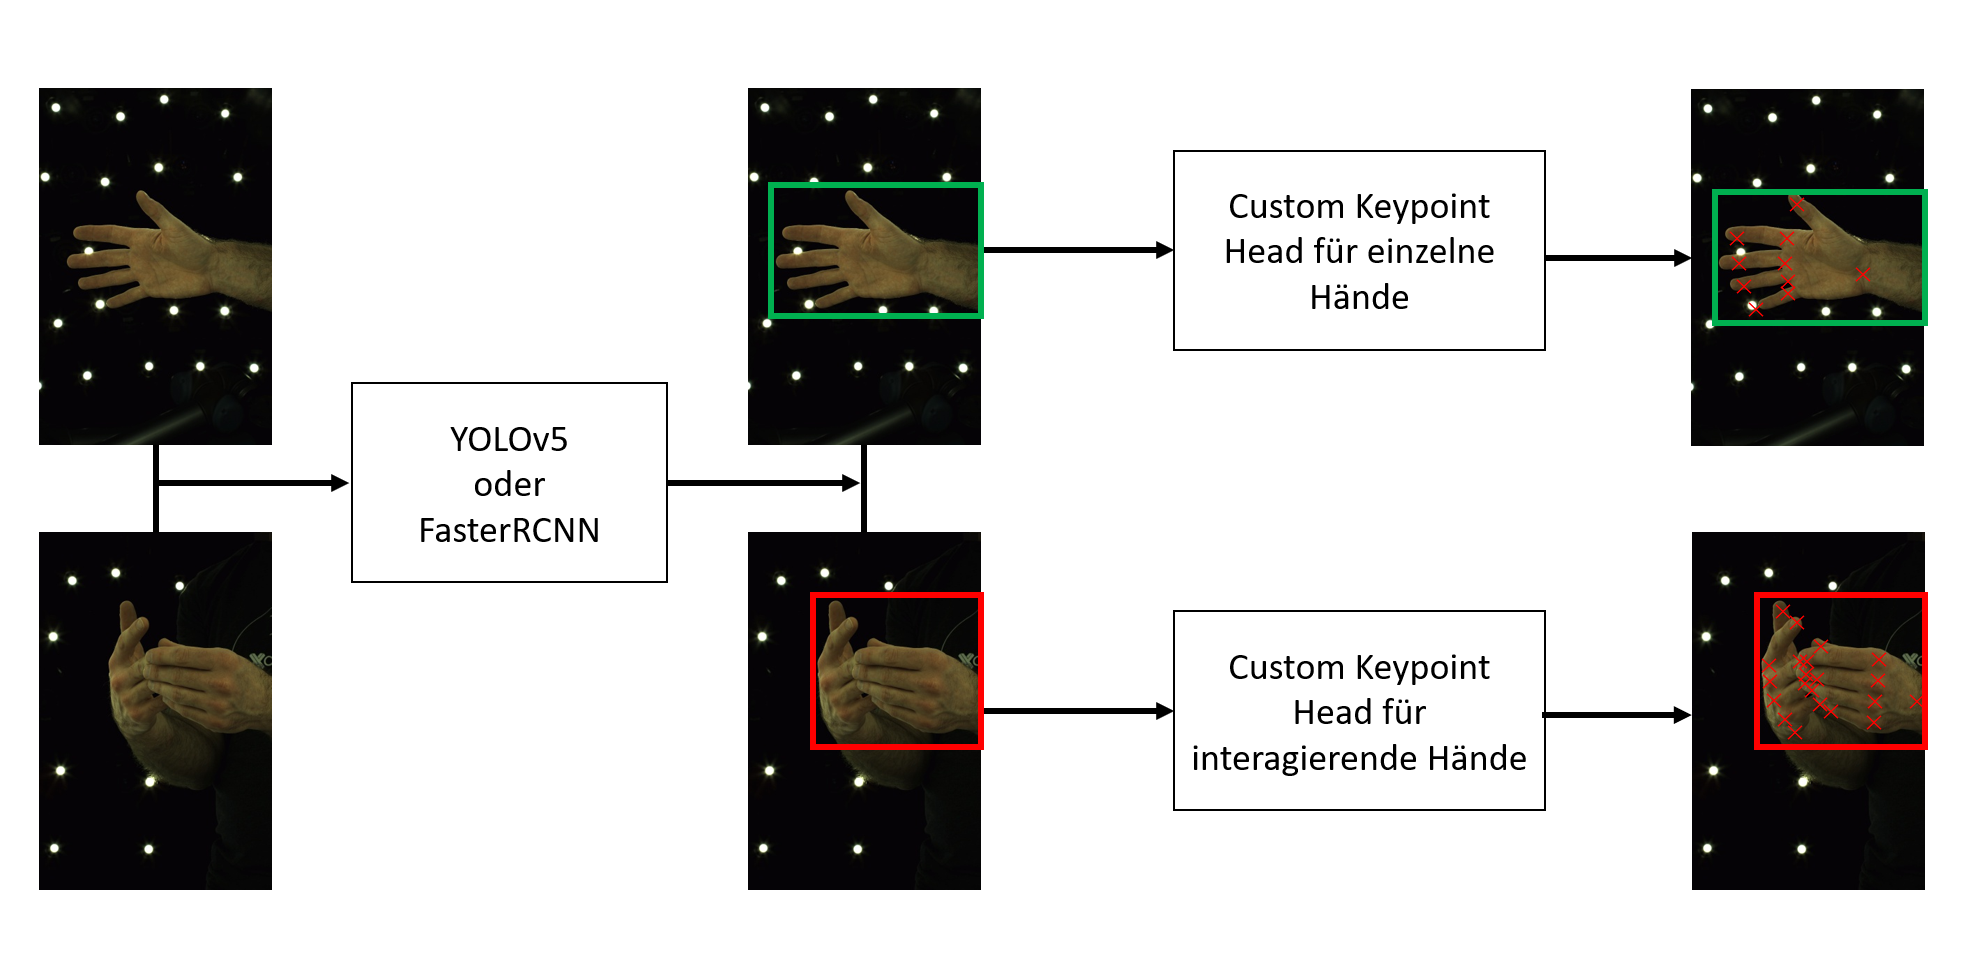
\includegraphics[width=15.5cm]{abbildungen/arch.PNG}}
    \caption{Übersicht Architektur}
    \label{fig:arch}
\end{figure} 

Als Alternative zu dieser Architektur, wird noch ein KeypointRCNN \cite{keypointrcnn} trainiert.
Dabei handelt es sich um Abwandlung von MaskRCNN, eine Weiterentwicklung der FasterRCNN Architektur, welche ursprünglich für Image Segmentation entwickelt wurde.
Diese Architektur wird detailliert in Kapitel \ref{ch:keypointrcnn} beschrieben.

\section{Dataset}\label{ch:dataset}
Die Bilder des InterHand2.6M Datensatz können über ein Python Skript, zu finden unter scripts/download\_data.py, heruntergeladen werden. 
Die Annotation müssen jedoch separat über die InterHand2.6M Website \cite{interhand_website} heruntergeladen werden. \\

Die Daten können als ein PyTorch Dataset geladen werden.
Dabei werden alle Annotationen geladen und vorverarbeitet. 
Während der Laufzeit werden die Bilder erst aus dem Filesystem geladen, was Ressourcen wie den Arbeitsspeicher schont. \\
\begin{lstlisting}[language=Python,caption={Dataset},label={lst:dataset},captionpos=b,showstringspaces=false, basicstyle=\small]
from dataset import dataset
data = dataset.Dataset(mode='train',
                    transform = None,
                    only_keypoints = False,
                    limit_handedness = 'all')
\end{lstlisting}
Die Keypoints der jeweiligen 2D Bilder sind nicht direkt in den Annotationen gespeichert.
Stattdessen sind Informationen über die Kameraposition (Kameramatrix) und die globalen 3D Koordinaten enthalten.
Mithilfe dieser, können die Keypoints auf das 2D Bild projiziert werden.\\
Über den Parameter 'mode' kann gesteuert werden, welcher der Datensätze (Train, Test oder Val) geladen werden soll.
Zusätzlich kann 'limit\_handedness' dazu genutzt werden, um nur Hände eines bestimmten Typs (interagierend, einzeln, links oder rechts) in dem Datensatz zu berücksichtigen.
Als Standard 'transform' wird eine Konvertierung zu einem PyTorch Tensor genutzt, jedoch kann bei Bedarf auch bspw. ein Resize übergeben werden.\\
Je nach Modell muss der Parameter 'only\_keypoints' gesetzt werden.
Ist dieser nicht gesetzt, so wird neben dem Bild als Input, ein Dict als Target übergeben.
Dieses ist im COCO Format \cite{coco} und enthält unter anderem Felder über die Bounding-Box der Hände, das Label der Hände und die Keypoints der Hände.\\
Ist der Parameter auf True gesetzt, so wird das Bild um die Bounding-Box herum ausgeschnitten.
Somit fällt der Großteil des Hintergrunds weg.
Zusätzlich werden die Keypoints der Hände normalisiert, d.h. diese haben einen Wert zwischen 0 und 1, je nachdem wie weit diese von den Rändern entfernt sind.
Ist das ausgeschnittene Bild zum Beispiel 500x500 Pixel groß und ein Keypoint befindet sich an Pixel [100 , 200] in diesem Ausschnitt, so wird dieser als [0.2 , 0.4] kodiert.\\

Das YOLOv5 Modell benötigt nicht als PyTorch Dataset, sondern in einer einzigen Ordnerstruktur.
Über das Skript scripts/create\_yolo\_annotations.py kann diese Ordnerstruktur erzeugt werden.
Jedoch benötigt dieser Vorgang ziemlich viel Zeit, da das Filesystem (Windows) nicht mit so viele Daten in einem einzigen Order zurechtkommt.
Die Erstellung des Val-Datensatzes mit ca. 380k Bildern benötigte nur eine halbe Stunde, wohingegen der Train-Datensatz knapp 45 Stunden brauchte, 90 mal solange trotz des eigentlich nur 3 mal so großen Datenmenge.

\section{YOLOv5}
YOLO steht für You Only Look Once, was auch direkt eine Besonderheit dieses Object Detection Networks ausmacht: Es reicht ein einziger Durchlauf des Bildes durch das Modell \cite{yolo1}.
In diesem Durchlauf, wird das Bild in ein Grid der Größe \textit{S x S} eingeteilt. 
Ist der Mittelpunkt einer Label-Bounding-Box in dieser Zelle, so ist diese Verantwortlich das Objekt zu erkennen.
Dabei werden \textit{B} Bounding Boxen in verschiedenen Größen und Längen-Breiten-Verhältnissen gebildet. 
Diese enthalten neben der Mittelpunkt, sowie Höhe und Breite der Box, noch den Confidence Score für entsprechendes Objekt.
Abbildung \ref{fig:yolo1_bbox} zeigt, wie diese Bounding Boxen auf einem Beispielbild aussehen.\\
\begin{figure}[!htb]
    \centering
    \fbox{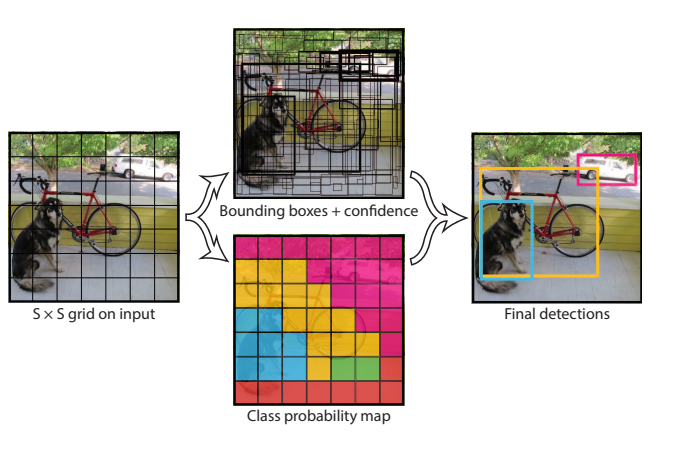
\includegraphics[width=10cm]{abbildungen/yolo1_bbox.PNG}}
    \caption{Bounding Box Erkennung YOLO \cite{yolo1} }
    \label{fig:yolo1_bbox} 
\end{figure} 

YOLO sagt dies Koordinaten dieser Bounding Boxen direkt im Forward-Pass des Modells vorher, was in der Architektur in Abbildung \ref{fig:yolo1_arch} ersichtlich ist.
Als Feature Network werden einige Convolution Layers genutzt, die anschließend als Input für Fully Connected Layers dienen. 
Diese FC Layers predicted dabei die Koordinaten der Bounding Boxes.\\
\begin{figure}[!htb]
    \centering
    \fbox{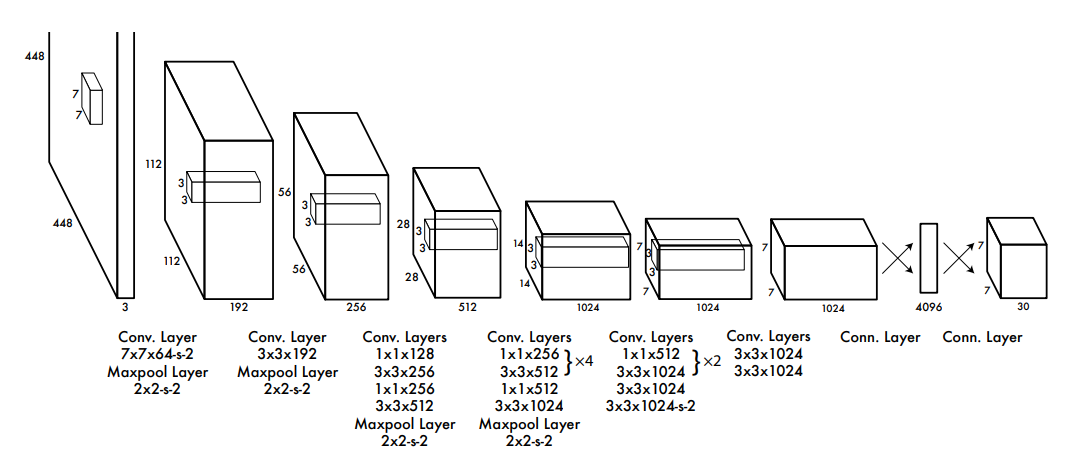
\includegraphics[width=15.5cm]{abbildungen/yolo1_arch.PNG}}
    \caption{Architektur YOLO \cite{yolo1} }
    \label{fig:yolo1_arch}
\end{figure} 

YOLOv5 ist eine Weiterentwicklung des ursprünglichen YOLO Modells.
Diese enthält diversen Verbesserungen, die teils auch über die vorherigen YOLO Varianten hinzugefügt wurden
So werden bspw. seit YOLO9000 (YOLO2) eine Optimierung der Bounding Box Vorschläge, sogenannte Anchor Boxen, genutzt \cite{yolo2}.
Die wichtige Neuerung von YOLO in Version Nummer 5 ist die Verwendung eines CSP Backbone.
Dabei handelt es sich um Convolutional Layers, bei denen einzelne Layers mehrfach verwendet werden.
Ziel dabei ist es, das Netzwerk dazu zu bringen Features wiederzuverwenden, sowie Probleme wie das Vanishing Gradient Problem zu verringern.\\

Um YOLOv5 zu trainieren, muss zuerst der Preprocessing Step aus Kapitel \ref{ch:dataset} ausgeführt werden.
Anschließend muss eine Konfiguration als .yaml Datei erzeugt werden, welche sich bereits unter yolo\_data/yolo\_dataset.yaml befindet.
Diese enthält neben den Pfad zu den Datensätzen auch die Labels der Klassen.
Nach dem Klonen des git-Repos, kann das Training über die Konsole gestartet werden.
Alternativ kann das Training auch über das Notebook Training.ipynb ausgeführt werden (dieses führt bei Bedarf auch nur den Konsolenbefehl aus).

\begin{lstlisting}[language=bash,caption={YOLO Training},label={lst:yolo_train},captionpos=b,showstringspaces=false, basicstyle=\small]
python .\yolov5\train.py --batch 2 --epochs 2 \\
    --data yolo_data/yolo_dataset.yaml \\
    --weights yolov5s.pt --freeze 8
\end{lstlisting}

\section{FasterRCNN}
Eine Alternative zu YOLO bietet die Klasse der RCNN Modelle.
FasterRCNN ist dabei der Nachfolger von FastRCNN und dieses wiederum von RCNN \cite{fasterrcnn}.
Im Gegensatz zu YOLO reicht es jedoch nicht, dass das Bild ein einziges Modell einmal durchläuft.
Stattdessen besteht FasterRCNN aus 3 Teilen: Feature Network, Region Proposal Network und einem Region of Interest Pooling. 
Abbildung \ref{fig:fasterrcnn} zeigt das Zusammenspiel dieser Komponenten. \\
\begin{figure}[!htb]
    \centering
    \fbox{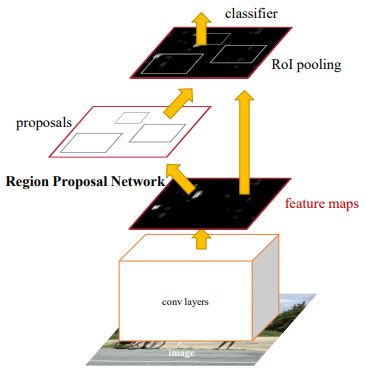
\includegraphics[width=10cm]{abbildungen/fasterrcnn_arch.PNG}}
    \caption{Architektur FasterRCNN \cite{fasterrcnn} }
    \label{fig:fasterrcnn}
\end{figure} 
Als Feature Network dienen einige Convolutional Layers. 
Hier können bereits vortrainierte Modelle (bzw. Convolution Layer dieser Modelle), bspw. ResNet50 genutzt werden.
Das Region Proposal Network (RPN) lässt sogenannte Anchor Boxen in verschiedenen Größe, Längen-Breiten-Verhältnissen und Ausrichtungen über das Bild laufen (wie ein Sliding Window).
Für jede dieser Anchor Boxen wird dabei predicted, ob ein Objekt darin enthalten ist (Vordergrund) oder nicht (Hintergrund).
Das Region of Interest Pooling (ROI Pooling) ist der letzte Schritt vor der Klassifikation.
Diese Schicht ist dabei ähnlich wie ein einfaches Max-Pooling.
Der Output des ROI Pooling kann nun als Input für einen Klassifikator genutzt werden, der die 'Vordergrund'-Objekte nun den richtigen Klassen zuordnet.\\

PyTorch bietet bereits eine Klasse für FasterRCNN Modelle an, welche auch in diesem Projekt genutzt wird.
Für dieses Modell wird ein Dataset im COCO-Format benötigt, welches bereits in \ref{ch:dataset} beschrieben wurde.
Das Notebook Training.ipynb enthält alle Schritte zur Erstellung, Anpassung und zum Trainieren des FasterRCNN Modells für Hände.

\section{Keypoint Head}

Sowohl YOLOv5 als auch FasterRCNN haben als Output eine Bounding Box um die Hände, sowie ein Label um welche Art von Hand (links, rechts oder interagierend) es sich handelt.
Um nun Keypoints zu bestimmen, wird ein neues Modell benötigt.
Dabei handelt es sich um ein Standard Convolutional Network, welches einige Convolutional Layers gefolgt von einigen Dense Layern beinhaltet.
Die Convolutional Layers werden dabei aber von einem VGG16-Net übernommen.
Die Fully Conected Layers werden von Grund auf an trainiert, wobei die Anzahl der Outputs der doppelten Anzahl der Keypoints entspricht.
Dies liegt daran, dass für jeden Keypoint eine x und eine y-Koordinate bestimmt wird.
Tendenziell wäre es möglich für jeden Hand Typen ein eigenes Modell zu trainieren, jedoch wurden lediglich 2 Modelle genutzt: Eines für interagierende Hände (42 Keypoints) und eines für einzelne Hände, egal ob linke oder rechte Hand (21 Keypoints).
Über entsprechende Parameter des PyTorch Dataset (siehe Kapitel \ref{ch:dataset}), wird das gecroppte Bild sowie die normalisierten Keypoints ausgegeben.
Diese werden bei diesen Modellen zum Training genutzt.
Als Loss Funktion wird hierbei ein simpler MeanSquarredError genutzt, als Optimizer dient Adam.

\begin{figure}[!htb]
    \centering
    \fbox{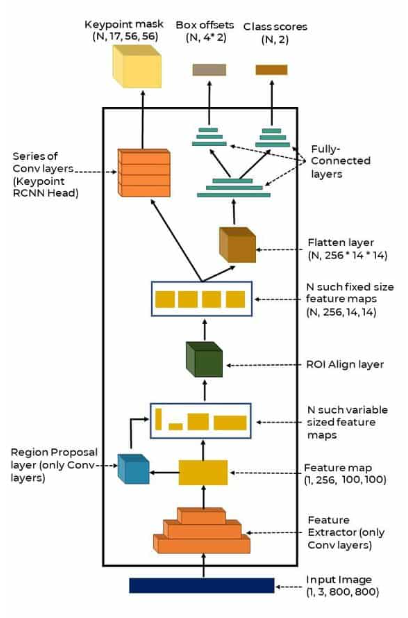
\includegraphics[width=10cm]{abbildungen/keypointrcnn_arch.PNG}}
    \caption{Architektur KeypointRCNN\cite{keypointrcnn_arch} }
    \label{fig:keypointrcnn}
\end{figure} 
\section{KeypointRCNN}\label{ch:keypointrcnn}
Eine Erweiterung der bereits beschriebenen FasterRCNN Architektur ist MaskedRCNN \cite{keypointrcnn}.
Es handelt sich dabei nicht zwingend um eine direkte Weiterentwicklung, da MaskedRCNN nicht für Object Detection sondern für Image Segmentation genutzt wird.
Dabei wird jeder Pixel einer entsprechenden Klasse zugeordnet.
MaskedRCNN baut jedoch auf der FasterRCNN Architektur auf mit einigen Anpassungen.
Anstelle der ROI Pooling Layer besitzt MaskedRCNN eine ROI Align Layer. 
Diese unterscheiden sich durch die Feinheit der weitergegeben Informationen: ROI Pooling nutzt den maximalen Wert, wohingegen ROI Align einen Mittelwert jedes Feldes bildet. 
Dadurch gehen weniger Informationen verloren.
Nach der ROI Align Layer, gibt es noch zusätzlich einen sogenannten MaskedRCNN Head.
Dabei handelt es sich um ein Fully Convolutional Network, bei dem jeder Channel des Outputs einer Klasse entspricht.\\
Eine Variation dieses Netzwerks ist das KeypointRCNN. 
Es besitzt die gleiche Architektur, jedoch ist der Output des MaskedRCNN Heads unterschiedlich.
Anstatt das jeder Channel eine Klasse repräsentiert, kodiert jeder Channel einen Keypoint. 
Abbildung \ref{fig:keypointrcnn} zeigt die Architektur eines KeypointRCNN bei dem 17 Keypoints eines Menschen aus dem COCO Datensatz predicted werden. \\
PyTorch bietet auch hier bereits eine Klasse für KeypointRCNNs an. 
Alle benötigten Schritte zur Modellerstellung und zum Training finden sich ebenfalls in dem Notebook Training.ipynb.


\section{Training}\label{ch:training}
Das Training fand parallel auf 2 Systemen statt: einem privaten Rechner mit einer RTX 2060 Super und einem Hochschulrechner mit einer RTX 2080 Super.
Da der Hochschulrechner eine geteilte Ressource ist, wurde das Training teilweise abgebrochen (z.B. wenn sich ein Student im Rahmen einer Vorlesung angemeldet hatte), wodurch das ganze Training neu gestartet werden musste.
Um solche Dinge zu vermeiden, wurde die Evaluierung mit dem Validation Datensatz bei FasterRCNN und KeypointRCNN weggelassen.
Beide Modelle trainierten für 4 Epochen, was beim FasterRCNN Modell knapp 100 Stunden und beim KeypointRCNN Modell knapp 200 Stunden benötigte. Auch die Custom Keypoint Modelle wurden nur über 5 Epochen trainiert.\\



  \chapter{Ergebnisse}

Die Evaluation wurde primär durch ausprobieren getestet. 
Das Notebook Visualize.ipynb enthält Funktionen um jede der Varianten zu visualisieren.

\section{YOLOv5}
YOLOv5 ist das Modell, welches in diesem Projekt am wenigsten optimiert wurde.
Dies lag an der hohen Trainingszeit, durch die hohe Auslastung des Filtersystems.
Es wurde ein YOLOv5s Modell (relativ kleines Modell) über 2 Epochen mit einigen Frozen Layern des Backbones trainiert.
Leider sind die Resultate von diesem nicht zu gebrauchen.
Es werden anstatt die selbst definierten Labels immer noch Objekte der Kategorie 'Person' erkannt, was vermutlich durch entsteht, dass es sich um ein vortrainierte Modell handelt.
Im weiteren Verlauf wurde deshalb FasterRCNN anstatt YOLO genutzt.

\section{FasterRCNN + Keypoint Head}
\begin{figure}[!htb]
    \centering
    \fbox{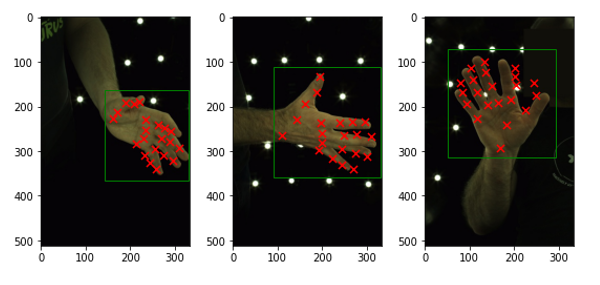
\includegraphics[width=15.5cm]{abbildungen/fasterrcnn_single_hand.PNG}}
    \caption{FasterRCNN+Keypoint Head, einzelne Hand}
    \label{fig:fasterrcnn_single}
\end{figure} 
Durch eine Aneinanderreihung des FasterRCNN Modells und der beiden Custom Keypoint Detection Heads, erhält man die beschriebene Architektur aus Kapitel \ref{ch:methods} (Abbildung \ref{fig:arch}).
Dabei detektiert FasterRCNN die Bounding Box der Hände sowie ob es sich dabei um einzelne oder interagierende Hände handelt.
Nachdem der Bildausschnitt innerhalb der Box ausgeschnitten wurde, wird dieses an entsprechendes Modell weitergegeben.
Die Keypoint-Predictions müssen jedoch vor der Visualisierung transformiert werden, da diese in einem Wertebereich zwischen 0 und 1 liegen.\\
Abbildung \ref{fig:fasterrcnn_single} zeigt einige gute Beispiele für die Erkennung einzelner Hände.
Die Keypoints sind relativ nah an den tatsächlichen Keypoints (Gelenken), jedoch oftmals einige Pixel versetzt.
Leider ist nicht jedes Ergebnis so gut, wie bei den dargestellten Beispielen.
Bei einigen Bildern sind die Keypoints geclustert in einer Ecke.
Jedoch ist der Ansatz vielversprechend und könnte durch zusätzliche Optimierungen, wie bspw Training mit mehreren Epochen, verbessert werden.\\

Anders sieht es jedoch bei interagierenden Händen aus,dort sind die Ergebnisse deutlich schlechter.
Wie in Abbildung \ref{fig:fasterrcnn_interagierend} sichtbar, sind die Keypoints oftmals geclustert.
Manchmal sind einige Keypoints auch in der oberen linken Ecke. 
Dies liegt daran, dass bei einigen Labels eine der beiden Hände fehlt, und alle Keypoints deshalb die Koordinaten (0,0) besitzen.
Durch mehrere und größere Schichten könnten sich die Ergebnisse verbessern.
Eine andere Alternative wäre es, zusätzlich noch Convolution Layers zu nutzen, welche die Keypoints als Heatmap lokalisieren, ähnlich wie bei KeypointRCNN.\\
\begin{figure}[!htb]
    \centering
    \fbox{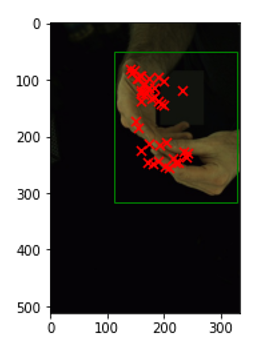
\includegraphics[width=5cm]{abbildungen/fasterrcnn_interacting.PNG}}
    \caption{FasterRCNN+Keypoint Head, interagierende Hände}
    \label{fig:fasterrcnn_interagierend}
\end{figure}


\section{KeypointRCNN}

Die besten Ergebnisse liefert KeypointRCNN. 
Da dieses Modell immer die gleiche Anzahl an Keypoints vorhersagt, wurde die Anzahl auf 42, 21 Keypoints pro Hand, gesetzt.
Abbildung \ref{fig:keypointrcnn_interagierend} zeigt einige Beispiele von interagierenden Händen.
Die Keypoints liegen sehr genau auf den Gelenken, welche durch diese kodiert werden.
Sogar wenn eine Hand die andere verdeckt (sichtbar in der Visualisierung rechts), werden die Keypoints der zweiten Hand korrekt dargestellt.\\
\begin{figure}[!htb]
    \centering
    \fbox{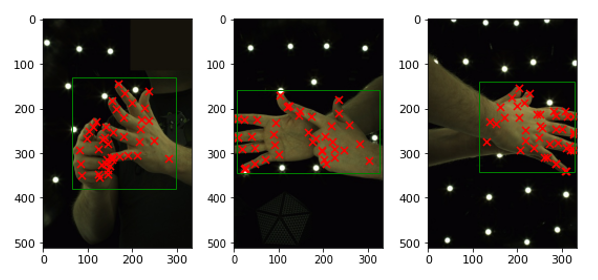
\includegraphics[width=15.5cm]{abbildungen/keypointrcnn_interacting.PNG}}
    \caption{KeypointRCNN, interagierende Hände}
    \label{fig:keypointrcnn_interagierend}
\end{figure} 
Sofern nur eine Hand im Bild ist, werden die Keypoints in der Regel aufeinander predicted, wie es Abbildung \ref{fig:keypointrcnn_single}. 
Dadurch sind es quasi 2 Keypoints pro Gelenk. 
In einem Post-Processing Schritt könnte man dies bei Bedarf raus filtern.
\begin{figure}[!htb]
    \centering
    \fbox{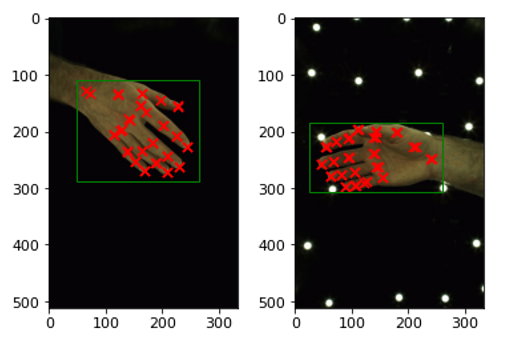
\includegraphics[width=10cm]{abbildungen/keypointrcnn_single.PNG}}
    \caption{KeypointRCNN, einzelne Hand}
    \label{fig:keypointrcnn_single}
\end{figure} 

  \chapter{Zusammenfassung}
KeypointRCNN Modelle sind eine großartige Möglichkeit sehr gute Ergebnisse im Bereich Keypoint Lokalisierung / Pose Estimation zu erhalten.
Durch die direkte Integration in PyTorch sind diese Modelle dazu auch sehr einfach zu erstellen und zu trainieren.\\
Eigene Modelle benötigen mehr Entwicklungsaufwand um vergleichbare Ergebnisse zu liefern, tendenziell sind diese sogar merklich schlechter.
Hier bietet es sich an, dass direkt in PyTorch verfügbare FasterRCNN  gegenüber YOLO zu bevorzugen. 
Eine Ausnahme bei der YOLO benutzt werden sollte, ist wenn die Echtzeit-Fähigkeit benötigt wird.
YOLO Modelle schaffen teilweise 100+ Frames pro Sekunde, wohingegen je nach Größe des FasterRCNN Modell, die Anzahl der Frames nur Zehntel beträgt.


  
  %\include{kapitel1}
  %\include{kapitel2}
  % ... weitere Kapitel
 
  % Literaturverzeichnis
  %\phantomsection
  %\addcontentsline{toc}{chapter}{Literaturverzeichnis}
  %\begin{thebibliography}{10}
  %  \bibitem{quelle1} Schreiberling, Tim: ,,Bestseller-Buch'', 1.~Auflage, S.~13ff, Renner-Verlag, Musterstadt, 2011.
  %\end{thebibliography}
  %\newpage
  
  % Literaturverzeichnis
  \bibliographystyle{wmaainf}
  \bibliography{refs}
  
  % Anhang
  \phantomsection
  \addcontentsline{toc}{chapter}{Abbildungsverzeichnis}
  \listoffigures
  \newpage
    
  \renewcommand{\lstlistlistingname}{Listingverzeichnis}  % change for German thesis
  \lstlistoflistings
  \newpage

  %\phantomsection
  %\addcontentsline{toc}{chapter}{Tabellenverzeichnis}
  %\listoftables
  %\newpage
  
  %\include{anhang}
\end{document}    